\documentclass[a4paper]{article}
\usepackage{fancyhdr}
\usepackage{amsmath}
\usepackage{xcolor}
\usepackage{graphicx}
\usepackage{latexsym}
\usepackage{amssymb}
\usepackage{listings}
\usepackage{array}

\lstset{basicstyle=\footnotesize,breaklines=true}

%%clickable links
\usepackage{hyperref}
\hypersetup{
    colorlinks=true, %colore les liens
    breaklinks=true, %permet le retour à la ligne dans les liens trop longs
    urlcolor= blue, %couleur des hyperliens
    linkcolor= black, %couleur des liens internes
}
%formatted algorithm:
\usepackage{algpseudocode}
\usepackage{algorithm}

\algblockdefx[Event]{Event}{EndEvent}%
[1][]{\textbf{Upon event :} #1}%
{}

\algblockdefx[Data]{Data}{EndData}%
[1][]{\textbf{Data :}}%
{}


\algblockdefx[Init]{Init}{EndInit}%
[1][]{\textbf{Initialization :}}%
{}


%% New commands
\newcommand{\eqdef}{\;\stackrel{\text{def}}{=}\;}

\begin{document}
\title{Distributed Systems: Network Simulator}
\author{David Beniamine \& Rodolphe Lepigre\\ MOSIG - Parallel, Distributed and Embedded Systems}

\date{\today}
\maketitle%affichage du titre
\begin{center}
    \tableofcontents%affichage de la table des matières
\end{center}
\newpage%commencement en page 2



%%%%%%%%%%%%%%%%%%%%%%%%%%%%%%%%%%%%%%%%%%%%%%%%%%%%%%%%%%%%%%%%%%%%%%%%%%%%%%
\section*{Introduction}
\addcontentsline{toc}{section}{Introduction}
As part of our Distributed Network class, we had to build a network simulator
tool and use it to implement and experiment with various broadcast protocols.
In particular we designed two regular total-order broadcast protocols and paid
much attention to the latency and throughput that they offer.

This report and the source files of the project are both part of our answer to
the problem. The source files should be globally well documented, but reading
this report should help the reader to better understand the structure of the
program.
\bigskip

\noindent\textbf{Structure of the report:} In the first section we present the
architecture and functionalities of our simulator. In particular the available
command line arguments are described. A Perl script is also provided with the
source files of the simulator. Its role is to help for the gathering of data
and automate the measurement of the the latency and the throughput of the
protocols. Its functioning is also explained at the end of the first section.

In the second and third sections we present two regular total-order broadcast
protocols. The first one achieves a good latency (time for a broadcast to be
completed with only one process sending), and the second one has a good
throughput when all process are sending at the same time. We give a detailed
theoretical analysis of the two protocols and confirm our results with some
experiments using the network simulator.

%%%%%%%%%%%%%%%%%%%%%%%%%%%%%%%%%%%%%%%%%%%%%%%%%%%%%%%%%%%%%%%%%%%%%%%%%%%%%%
\section{The network simulator}
In this section we describe the architecture of the network simulator that we
programmed using the C programming language. The simulator follows a round
based approach and makes use of only one thread, as was part of its
specification.

\subsection{Basic principle and usage}
Before diving into a detailed description of the architecture of the program,
we will start by giving some hints on how to use the simulator, and also try
to provide some intuition to the reader on its basic working principles.

Let us first outline some useful terminology that we will use throughout this
report. In our simulator, a single machine capable of sending a message to
other machines will be called a \textit{process}, a \textit{node}, or simply
a \textit{machine}. The term \textit{external event} will refer to any action
taken by the user of the simulator. For example, at some point the user might
decide that a node should initiate a broadcast. This information will be
passed to the program using an external event.

Before being able to use the simulator, the user should first compile it. A
\textit{makefile} is provided in the source directory \textit{src/}. It is
considered that the user is running a \textit{POSIX}-friendly operating system
and that the regular building tools are present on his machine (\textit{gcc},
\textit{make},...).
\begin{lstlisting}
> cd src/
> make
\end{lstlisting}

Once the program has been (successfully) compiled, an executable file should
have appeared in the source directory. The program contains a ``help'' section
which can be accessed in a standard manner.
\begin{lstlisting}
> ./Broadcast -h
Usage: ../src/Broadcast [-N n][-R n][-h][-b|t|p|L|T]
Possible arguments:
-N n	Specify a number of nodes n, default is 4.
-R n	Specify a number of rounds n, default is 20.
-h	Display this help message.
Selection of broadcast mode:
-b	Basic broadcast (default).
-t	Tree broadcast.
-p	Pipeline broadcast.
-L	Total order broadcast with good latency.
-T	Total order broadcast with good throughput.
\end{lstlisting}

The behaviour of the program can be changed using the command line arguments
as hinted by the ``help'' section content. In particular, the number of nodes
and the number of rounds to run can be set (if the number of round is set to
$0$ the system will run forever).

The broadcast protocol that is going to be used can be selected from the
command line as well. The available options are the following.
\begin{itemize}
    \item Basic broadcast: the broadcaster sends to every other node in turn
        (one per round).
    \item Tree broadcast: messages are send on a tree. The broadcaster is the
        root, and nodes forward the messages to their children.
    \item Pipeline broadcast: the broadcaster sends the message to its neighbour
        which sends it to its neighbour and so on.
    \item Total order broadcast with good latency (see section
        \ref{sec:latencyTO}).
    \item Total order broadcast with good throughput (see section
        \ref{sec:throughputTO}).
\end{itemize}

Once the program is run, the simulation starts right away. At each turn, the
user will be prompted to enter external events for the system. Any number of
external event can be entered at the beginning of each round. External events
are read on the standard input (one by line). And when the user is done
sending events, he should simply type ``start'' for the simulator to do a
round. The format for the external events is the following.
\begin{lstlisting}
id event
\end{lstlisting}
``id'' is an integer between $0$ and $N-1$ where $N$ is the number of nodes in
the system. This field allows the system to know to which node the external
event is destined.

``event'' is the content of the event passed to the node which can be an
arbitrary string (with no line break).

The only event that is available (for now) is called ``broadcast'' and tells
the system that the referenced node should broadcast the message ``Hello''.

Of course the user can use a file and pipe it to the standard input of the
program. This is the most convenient way to run tests and experiments. An
example of the content of such file is the following.
\begin{verbatim}
0 broadcast
start
start
start
start
start
start
\end{verbatim}
This example file can be used to measure the latency of a protocol for
example.

\subsection{Architecture of the system}
In order to better understand how the source code is organized, we give a
brief description of the content of every source file.
\begin{itemize}
    \item \textit{List.h} define the structure List used by
        \textit{Fifo.$<$c/h$>$} and \textit{SortedList.$<$c/h$>$}
    \item \textit{SortedList.h} contains a small library providing sorted list
        of objects. This library can be used by the nodes to store and sort
        their messages.
    \item \textit{SortedList.c} implements the functions defined in
        \textit{SortedList.h}
    \item \textit{Fifo.h} contains a small library providing queues. These are
        used to store pending messages of external events for each process.
        It seems fair for messages (resp. external events) to be sent (resp.
        treated) in the order they arrived in the system (FIFO order: First
        In, First Out).
    \item \textit{Fifo.c} implements the functions defined in \textit{Fifo.h}.
    \item \textit{Message.h} defines what messages (a sender, a receiver and
        the content) and provides functions to initialize, delete and copy
        messages.
    \item \textit{Message.c} implements the functions defined in
        \textit{Message.h}.
    \item \textit{Broadcast.h} contains a definition of the different
        broadcast protocols.
    \item \textit{Broadcast.c} implements all the different broadcast
        protocols.
    \item \textit{Simulator.h} defines the core functions and data structures
        of the simulator accessible by the nodes or the main function. In
        particular the function \textit{LaunchSimulation} is the core function
        of the simulator and contains the main loop which will do the rounds,
        read external events and apply the broadcast policies defined in
        \textit{Broadcast.h}.
    \item \textit{Simulator.c} defines the internal structure of the simulator
        and implements the functions defined in \textit{Simulator.h}.
    \item \textit{Main.c} contains the main function of the program. It takes
        care of the command line arguments, initialize the system and call the
        \textit{LaunchSimulation} function.
\end{itemize}

\subsection{Implementing a protocol with the simulator}
Our simulator provides a convenient way to implement broadcast protocols. The
main part of the process is the creation of a function having the following
signature.
\begin{verbatim}
void myProtocol(int id, Message m);
\end{verbatim}

This function will be run by each node at each round of the execution with its
first argument containing the identifier of the current node and the second
argument being the message received by the current node at the beginning of the
round (or NULL if it is not receiving any message).

The function should be placed in file \textit{Broadcast.c} and its signature
should be added to \textit{Broadcast.h}. In order to launch the simulator with
the newly created function a main program should be written as well. The main
function included in \textit{Main.c} can be modified easily to be made to use
the new protocol function. Alternatively the following is an example of a
main program.

\begin{verbatim}
#include "Broadcast.h";
#include "Simulator.h";

#define NB_NODES 4
#define NB_ROUNDS 20

int main(void){
  // Initialize the system
  initSytem(NB_NODES, NB_ROUNDS, myProtocol);

  // Run the simulator
  LaunchSimulation();

  // Delete the system
  deleteSystem();

  return 0;
}
\end{verbatim}

A node can interact with the systems using the functions defined in
\textit{Simulator.h} and \textit{Message.h}. For instance the function
\textit{readExternalEvent} is provided in order to get the next external
event if there is any. There is also a \textit{Send} function that is used to
add a message in the sending queue of a process. There is also a function
to get the number of nodes in the system and some other allowing to attach
some persistent data to a node, retrieve it and modify it. Here is an example
of a data structure that can be held in a node as persistent data.
\begin{verbatim}
typedef struct _NodesData{
    int clock;
    SortedList pending;
}*NodesData;
\end{verbatim}
The following functions are used to set the stored data and to retrieve it.
\begin{verbatim}
void *setData(int id, void *data);
void *getData(int id);
\end{verbatim}

Note that messages can be sent either as a unicast (from one node to one other
node) or as a multicast (from one node to all the other nodes), but the
multicast is not reliable, it is very similar to the IP broadcast. A message
multicasted when its destination address is set to $-1$.

Once the protocol is ready, the Perl script can be used to gather statistics.

\subsection{Experimental script}
For the experiments to be easily reproduced, we provide a Perl script
\textit{exp.pl} with our simulator, which allows the user to run every
experiment presented in this report.

This script runs the program \textit{Broadcast} with different numbers of
nodes and displays the latency and the throughput for each runs. If the reader
wishes to use the script, he is advised to run it with the ``-h'' argument to
display the ``help'' section.

\begin{lstlisting}
> ./exp.pl -h
\end{lstlisting}

%%%%%%%%%%%%%%%%%%%%%%%%%%%%%%%%%%%%%%%%%%%%%%%%%%%%%%%%%%%%%%%%%%%%%%%%%%%%%%
\section{Regular total-order broadcast protocols with good latency}
\label{sec:latencyTO}

This first protocol makes use of the tree broadcast protocol since it achieves
an optimal latency of $log(n)$. In order to obtain a total-order, i.e.
guarantee that any two process will deliver messages in the exact same order,
we use one of the nodes as a relay. More precisely, when a node wishes to
perform a broadcast, it sends the message to the relay node which will
broadcast the message on its behalf.

Intuitively, all nodes in the tree will receive the messages in the same order
since the same tree traversal scheme will be used for each message. When a
node of the tree receives a broadcasted message, it can deliver it immediately
before forwarding it.

Since the messages to be broadcasted need to be sent to the relay node, the
achieved latency should be equal to the latency of the tree broadcast plus
the time required to unicast a message (which is $1$ round). Hence, the
latency of this protocol should intuitively be $log(n) + 1$ rounds.

\subsection{Algorithm}
\begin{algorithm}[H]
    \centering
    \begin{algorithmic}[5]
        \Data
        \State int[][] Children
        \Comment{Ordered list of the childrens of each nodes}
        \EndData
        \Init
        \For{n in AllNodes()}
        \State Children[n]$\gets\{(2n + 1)2^i | i \in \mathbb{N}\} \cap \text{AllNodes()}$
        \Comment{Children[n] is sorted in increasing order}
        \EndFor
        \EndInit
        \Event $< tob,Broadcast\ |\ m> $
        \Comment{Start a broadcast}
        \If{Id()==0}
        \Comment{If the broadcaster is the relay}
        \State Deliver(0,m)
        \Comment{It can deliver}
        \For{c in Children[0]}
        \Comment{And forward the message}
        \State Send(c,$<m,0>$)
        \EndFor
        \Else
        \Comment{Otherwise ask the relay to forward}
        \State Send(0,$<m,Id()>$)
        \EndIf
        \EndEvent

        \Event $<Receive\ | <m,broadcaster>>$
        \State Deliver(broadcaster,m)
        \Comment{Deliver right away}
        \For{c in Children[Id()]}
        \Comment{And forward the message}
        \State Send(c,$<m,broadcaster>$)
        \EndFor
        \EndEvent
    \end{algorithmic}
    \caption{Tree-based total ordered broadcast protocol}
\end{algorithm}

\subsection{Theoretical analysis}
\subsubsection{Correctness}
\noindent\textbf{Validity.} We assume that there are no crashes, so if a
process $p$ broadcasts a message $p$, then $p$ eventually delivers $m$. If
$p = 0$ ($p$ is the relay node) the proof is trivial (by definition of the
\textit{Broadcast} event).

If $p$ is not the relay, the message $m$ will be forwarded to the  relay for
it to perform the broadcast. Since the broadcast is propagated on a tree which
root is the relay, any node in the tree will eventually deliver the message
(by definition of the \textit{Receive} event). In particular $p$ will
eventually deliver it.

\bigskip
\noindent\textbf{No duplication.} When a message is broadcasted by a node $p$
it is not delivered right away by $p$ (except if $p = 0$). A node $p$ only
delivers a message $m$ when it receives it from its parent node (by definition
of the \textit{Receive} event). By the property that no node in a tree can
have more than one parent, a message can only be delivered once.

\bigskip
\noindent\textbf{No creation.} Delivery of message $m$ by a process $p$ happen
in two cases. Either during a \textit{Broadcast} event if $p=0$, or during a
\textit{Receive} event.

In the first case, the message $m$ is delivered by process $p=0$, which
initiated itself a broadcast (the message $m$ was previously  broadcasted by
process $p=0$).

In the second case, the message $m$ is delivered by $p$ in response to a
\textit{Receive} event. As we are using a perfect point-to-point link (with in
particular no creation), the message was sent by the parent of the node, which
received it previously by its parent and so on up to the root of the tree, which
is process $0$. There are two possibilities: either $0$ is the broadcaster, or
not. In the first case $0$ previously initiated the broadcast. In the second
case, some other process $s$ initiated the broadcast and sent its message to
the relay (by definition of the \textit{Broadcast} event).

\bigskip
\noindent\textbf{Agreement.} Since all process are correct (no crashes) we need
to show that when a message $m$ is delivered by a process $p$ then it is
eventually delivered by every other process. Processes are organized in a tree
which root is process $0$, so process $p$ has related nodes in the tree: a
parent if $p \neq 0$, siblings and children.

If $p \neq 0$, his parent should have delivered message $m$ before $p$ since
the message was forwarded to $p$ by its parent.

If $p$ has siblings (nodes that share the same parent as $p$), the parent
should take care of forwarding the message to them, and the message will be
properly delivered in the sibling branches of the tree independently of what
happens for $p$.

If $p$ has children it will eventually forward message $m$ to them (by
definition of the \textit{Receive} event) so that they can deliver it and
forward it in turn to their children and so on.

\bigskip
\noindent\textbf{Total order.} All the messages are effectively broadcasted by
process $0$ (the relay) since no delivery happens until process $0$ receives
the message to broadcast. Once process $0$ has chosen an order for the
messages to be delivered, the order of delivery is kept throughout the tree.
Since every node has only one parent and the link between this node and its
parent is FIFO, there can be no inversion. Also when a node forwards a message
to its children it sends this message to all of its children without
interleaving other messages during the process. This ensures a total order
for the delivery of messages.

\subsubsection{Latency}
The algorithm is based on the tree-broadcast protocol seen in class. This
protocol has a latency of $\lceil\log_2(N)\rceil$ where $N$ is the number of
nodes.

The protocol presented in this section makes use of the tree-broadcast
protocol by having a node called the relay broadcast all the messages on
behalf of all the nodes of the system (and in particular itself).

When the relay originates a broadcast, the latency is that of the tree
broadcast protocol, i.e. $\lceil\log_2(N)\rceil$. However, when a node that is
not the relay wished to broadcast a message, it first needs to unicast the
message to the relay, which take one round. The latency is then
$\lceil\log_2(N)\rceil + 1$. To better understand what happen, two examples
of broadcasts in a system with four nodes are displayed in Figure
\ref{figure:latency}. The first broadcast is performed by the relay and the
second by an other node.

\begin{figure}[h]
    \centering
    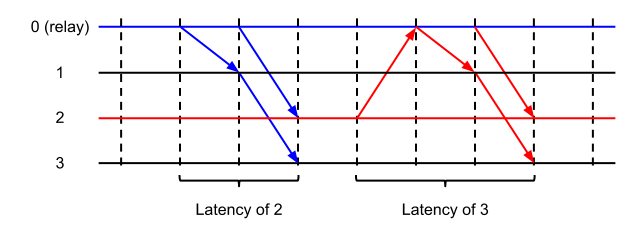
\includegraphics[width=280px]{Latency.png}
    \caption{an example of broadcast from the relay (blue) and an example of broadcast from an other node (red).}
    \label{figure:latency}
\end{figure}

We give two different results for the latency:
\begin{itemize}
    \item \textbf{Worst case latency:} $\lceil\log_2(N)\rceil + 1$
    \item \textbf{Mean latency:} $\frac{1}{N} \lceil\log_2(N)\rceil +
        \frac{N-1}{N} (\lceil\log_2(N)\rceil + 1)
        = \lceil\log_2(N)\rceil + \frac{N-1}{N}$
\end{itemize}

Both the worst case and the mean latency tend to the optimal when $N$ is
large.

\subsubsection{Throughput}
Let's consider a system with $N$ nodes that wishes to broadcast a message
concurrently. We wish to know how long this will take for all $N$ broadcasts
to complete.

At the first step, the relay only knows of the message it wishes to broadcast
so it starts to broadcast it. After $\lceil\log_2(N)\rceil$ steps, the relay's
broadcast is completed.

In the mean time, the relay has been sending data but has had plenty of time
to receive the data to broadcast from one of the other nodes. The second tree
broadcast from $0$ can hence start right away, and is completed after
$\lceil\log_2(N)\rceil$ steps.

By reasoning in the same way we can see that it takes $N \lceil\log_2(N)\rceil$
rounds to complete the $N$ broadcasts. This gives us the throughput of the
system which is equal to $\frac{1}{\lceil\log_2(N)\rceil}$.

The throughput tends slowly to $0$ when $N$ grows large, which is quite bad.

An example of a system where four nodes are concurrently broadcasting a message
is displayed in Figure \ref{figure:throughput}.

\begin{figure}[h]
    \centering
    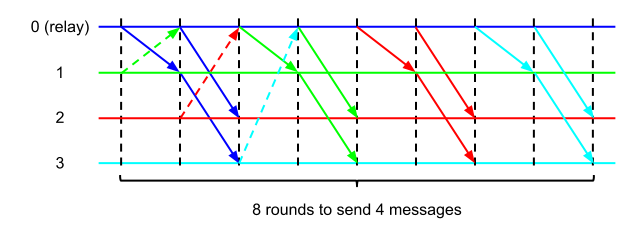
\includegraphics[width=280px]{Throughput.png}
    \caption{Four nodes broadcasting a message concurrently. Node 0 is the relay, it effectively performs all broadcasts using the tree broadcast protocol. The dashed arrows are request for a broadcast from nodes to the relay.}
    \label{figure:throughput}
\end{figure}

We see on the drawing that the relay can perfectly receive messages from the
other nodes while playing its role in the broadcast.

\subsection{Empirical analysis}
The empirical evaluation of the protocol are done using the network simulator.

\subsubsection{Latency}
In order to evaluate the latency of the protocol with the network simulator,
we run tests where a single node broadcasts a message and repeat the experiment
with different number of nodes. We then see how many rounds it takes for the
broadcast to be completed in each system.

We ran two different experiments. In the first one, the sender is always the
relay, so we expect a latency of $L_{\text{relay}} = \lceil\log_2(N)\rceil$.
The second experiment is the same, but the node that is broadcasting is not
the relay. In this case the expected latency is
$L_{\text{node}} = \lceil\log_2(N)\rceil + 1$. The results are displayed in
Table \ref{table:la}.

\begin{table}[H]
    \centering
    \begin{tabular}{|c|c|c|c|c|}
        \hline
        $N$  & $L_{\text{relay}}$ & $\lceil\log_2(N)\rceil$ & $L_{\text{node}}$ & $\lceil\log_2(N)\rceil + 1$ \\
        \hline
        1     & 0    & 0    & -    & -    \\
        2     & 1    & 1    & 2    & 2    \\
        3     & 2    & 2    & 3    & 3    \\
        4     & 2    & 2    & 3    & 3    \\
        5     & 3    & 3    & 4    & 4    \\
        6     & 3    & 3    & 4    & 4    \\
        7     & 3    & 3    & 4    & 4    \\
        8     & 3    & 3    & 4    & 4    \\
        9     & 4    & 4    & 5    & 5    \\
        10    & 4    & 4    & 5    & 5    \\
        100   & 7    & 7    & 8    & 8    \\
        1000  & 10   & 10   & 11   & 11   \\
        %    10000 & 14   & 14   & 15   & 15   \\
        \hline
    \end{tabular}
    \caption{Protocol latency with different number of nodes with the broadcasting node being the relay or not.}
    \label{table:la}
\end{table}

The results are exactly the one expected and confirm the validity of the
theoretical analysis. Note that there must always be a relay in the system, so
when there is only one node, it has to be the relay. Hence it makes no sense
for a node that is different from the relay to broadcast a message if there is
only the relay in the system.

\subsubsection{Throughput}
We experiment with the throughput in the same way as with the latency. We use
the simulator to run test where every node in the system has a message to
broadcast from the beginning of the run. We then see how long it take for all
the broadcasts to be completed. The expected throughput is
$\frac{1}{\lceil\log_2(N)\rceil}$ where $N$ is again the number of nodes in
the system. The results are displayed in Table \ref{table:thr}.

\begin{table}[H]
    \centering
    \begin{tabular}{|c|c|c|}
        \hline
        $N$   & $T$  & $\frac{1}{\lceil\log_2(N)\rceil}$ \\
        \hline
        1     & +Inf   & +Inf   \\
        2     & 1.0    & 1.0    \\
        3     & 0.5    & 0.5    \\
        4     & 0.5    & 0.5    \\
        5     & 0.333  & 0.333  \\
        6     & 0.333  & 0.333  \\
        7     & 0.333  & 0.333  \\
        8     & 0.333  & 0.333  \\
        9     & 0.25   & 0.25   \\
        10    & 0.25   & 0.25   \\
        100   & 0.143  & 0.143  \\
        1000  & 0.1    & 0.1    \\
        %    10000 & 0.071  & 0.071  \\
        \hline
    \end{tabular}
    \caption{Protocol throughput with different number of nodes, all nodes broadcasting a message concurrently}
    \label{table:thr}
\end{table}

The results fit exactly the theoretical model. We observe, as expected, that
the relay starts its broadcast first (since it has its own message to
broadcast from the beginning) and the nodes manage to send messages to
broadcast to the relay while it is still performing the previous broadcast.
With this, the throughput of $\frac{1}{\lceil\log_2(N)\rceil}$ is achieved.

Note that with only one node the throughput is infinite since it take no time
for the node to broadcast a message (it already has it).

%%%%%%%%%%%%%%%%%%%%%%%%%%%%%%%%%%%%%%%%%%%%%%%%%%%%%%%%%%%%%%%%%%%%%%%%%%%%%%
\section{Regular total-order broadcast protocol with good throughput}
\label{sec:throughputTO}
This protocol is based on the pipeline broadcast, but to ensure the total order
property we add a reverse pipeline for the acknowledgement. The idea is that if
a node $p$ is able to deliver a message, every other process have been a part of
the pipeline sending $m$ or it's acknowledgement to $p$. As a node can receive
a message from different process, we also add a sorted list of message, and we
ensure that a process can deliver a message $m$, only if $m$ is acknowledged
and $m$ is at the head of the list.

It's clear that as a message have to go through two pipelines, the latency will
be of the order of $2N$ (where $N$ is the number of process). But we use
reversed pipeline for the acknowledgement, the can be sent in parallel and it
takes also about $2N$ rounds to broadcast $N$ different nodes, so we are able
to achieve a constant throughput of $\frac{1}{2}$.

\subsection{Algorithm}
\begin{algorithm}[H]
    \centering
    \begin{algorithmic}[5]
        \Data
        \State unsigned int : clk
        \Comment{A logical clock}
        \State unsigned int : next
        \Comment{the id of the next process in the pipeline}
        \State unsigned int : prec
        \Comment{the id of the previous process in the pipeline}
        \State Pending : OrderedList
        \Comment{A list ordered by clock then id}
        \EndData
        \Init
        \State clk$\gets$0
        \State next$\gets$(Id()+1)\%NProcess
        \State prec$\gets$(Id()-1)\%NProcess
        \State Pending$\gets$EmptyQueue
        \EndInit
        \Event $< tob,Broadcast\ |\ m> $
        \Comment{Start a broadcast}
        \State clk++;
        \If{next$\ne$Id()}
        \Comment{We are not the only node of the system}
        \State Pending$\rightarrow$add($<m,Id(), clk, false>$) 
        \Comment{The message is added\\}
        \Comment{to the list the false boolean\\}
        \Comment{indicate that we have to wait for one ack}
        \State Send(next,$<m,Id(),clk>$)
        \Else
        \Comment{We are the only node of the system}
        \State{Deliver(Id(),m)}
        \EndIf
        \EndEvent
        \Event $<Receive\ | <m,sender, mclk>>$
        \State clk$\gets$MAX(clk, mclk)+1
        \If{next=sender}
        \State Pending$\rightarrow$add($<m,sender,mclk,true>$)
        \Comment{We are at the end\\}
        \Comment{of the pipeline}
        \State Send(prec,$<ack,sender,mclk>$)
        \Comment{so we start the\\}
        \Comment{broadcast of acks}
        \If{Pending$\rightarrow$IsHead(sender,mclk)}
        \State Pending$\rightarrow$RemoveHead()
        \Comment{m is the first message of\\}
        \Comment{the queue, we can deliver it}
        \State Deliver(sender,m)
        \Comment{And deliver it}
        \EndIf
        \Else
        \State Pending$\rightarrow$add($<m,sender,mclk,false>$)
        \State Send(next,$<m,sender,mclk>$)
        \Comment{We forward m\\} 
        \Comment{through the pipeline}
        \EndIf
        \EndEvent
        \algstore{myalg}
    \end{algorithmic}
    \caption{Pipeline based total ordered broadcast protocol}
\end{algorithm}
\begin{algorithm}[H]
    \centering
    \begin{algorithmic}[5]
        \algrestore{myalg}

        \Event $<Receive\  | <ack,sender, mclk>>$
        \State clk$\gets$ Max(clk,mlck)+1
        \If{sender$\neq$Id()}
        \Comment{We have to forward the ack}
        \State Send(prec,$<ack,sender,mclk>$
        \EndIf
        \If{Pending$\rightarrow$IsHead(sender,mclk)}
        \Comment{m is the head\\}
        \Comment{we can deliver it}
        \State m$\gets$(Pending$\rightarrow$RemoveHead())
        \State Deliver(sender,m)
        \State $<m,sender,mclk,b>\gets$Pending$\rightarrow$getHead()
        \While{b}
        \Comment{While we have receive an ack for\\}
        \Comment{the message at the head of the queue\\}
        \Comment{we can deliver it}
        \State Pending$\rightarrow$RemoveHead()
        \State Deliver(sender,m)
        \State $<m,sender,mclk,b>\gets$(Pending$\rightarrow$getHead())
        \EndWhile
        \Else
        \Comment{m isn't the head we mark m as acknowledged\\}
        \Comment{but deliver it until m is the head\\}
        \Comment{of the pending queue}
        \State Pending$\rightarrow$Remove($<m,sender,mclk,false>$)
        \State Pending$\rightarrow$Add($<m,sender,mclk,true>$)
        \EndIf
        \EndEvent
    \end{algorithmic}
\end{algorithm}


\subsection{Theoretical analysis}
\subsubsection{Correctness}
\label{sec:pipelineack-proof}
\noindent\textbf{Validity.} As there is no crashes, if a process $p$
broadcasts a message $m$, it will be received, put in the pending queue and
acknowledged by every process. When $p$ receives the ack for $m$, either $m$
is the head of the queue and in that case $p$ delivers it, or $p$ will have
to wait for at least one other ack message.

As the queue is ordered by logical clock and as all nodes have been on the
pipeline forwarding $m$ or it's ack, once $p$ has received the acknowledgment
for $m$, no new message will be able to go before $m$ in the queue. Finally as
all message will eventually be acknowledged, so the number of message before
$m$ in the queue will decrease. And at one moment, after the reception of one
ack, $m$ will be the head of the queue and will be delivered.

So if $p$ broadcasts a message $m$, it will eventually receive an ack for $m$
and deliver it.

\bigskip
\noindent\textbf{No duplication.} Each message is sent and ack only once. As
soon as a message is delivered it is removed from the pending queue. To be
delivered, a message needs to be the head of the pending queue, as we remove a
message of this queue as soon as we deliver it, we cannot deliver a message
twice.

\bigskip
\noindent\textbf{No creation.} No rules of the algorithm allow a process to
create a message $m$ without receiving a broadcast request for $m$.

\bigskip
\noindent\textbf{Agreement.} We have proved that if $p$ broadcast a message
$m$ then $p$ will eventually receive an ack for $m$ and deliver $m$, as the
pipeline go through all the nodes and as a node deliver a message as soon as
it acknowledge it, if $p$ delivers $m$ every node have delivered $m$.

\bigskip
\noindent\textbf{Total order.} Let us imagine that process $p_1$ has delivered
message $m_1$ before message $m_2$ and that process $p_2$ has delivered
message $m_2$ before message $m_1$.

As all the node's queues are sorted the same way we can consider that the
\textit{right} order is the order of the queue, and we (arbitrarilly) state
that this order is $m_1 < m_2$.

So if $p_2$ has delivered $m_2$ before $m_1$, this means that $p_2$ had
received $m_2$, delivered it, and then received $m_1$. Indeed if $m_1$ have
been received before $m_2$ or if $m_1$ and $m_2$ have been in the queue at the
same time, $p_2$ would have delivered $m_1$ before $m_2$.

Either $p_2$ is the last node of the pipeline used by $m_1$, or $p_2$ has
received an ack for $m_1$. In both cases, this means that when $p_2$ is able
to deliver $m_1$, all the process have seen $m_1$ and done the operation 
\textit{clock=Max(clock(m1),MyClock)+1} before forwarding it or sending an
ack. If a process had send $m_2$ with a clock smaller or equal to
\textit{clock(m1)}, this message would have used the same path than $m_1$
(or $m_1$'s ack) and as the link are FIFO, $p_2$ would have received $m_2$
before $m_1$. This contradict the hypothesis so two process can't deliver two
message in a different order.

\subsubsection{Latency}
The algorithm is based on the pipeline broadcast, if we have $N$ nodes, it takes
$N-1$ round for one broadcast. But as the last node of the pipeline start a
broadcast of acknowledgment, and as we wait for these ack to deliver the
message, the message is delivered by all the nodes only after $2(N-1)$ rounds.

Figure \ref{figure:latency2} shows a broadcast on 4 nodes. We can see that
we have a Latency of $6=2*(4-1)$.

\begin{figure}[h]
    \centering
    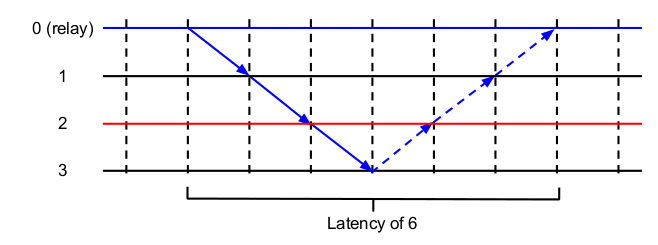
\includegraphics[width=280px]{Latency2.png}
    \caption{One node broadcasting on the pipeline. The dashed arrows are
    acknowledgements}
    \label{figure:latency2}
\end{figure}

As the two pipelines are symmetrical, we will be able to parallelize broadcast
during the sending and during the acknowledgement phases, so we will be able to
keep this latency of $2(N-1)$ while sending $N$ messages.
\subsubsection{Throughput}
Let’s consider a system with N nodes that wishes to broadcast a message concurrently
We wish to know how long this will take to all N broadcasts to
complete.

As shown in Figure \ref{figure:throughput2}, all the nodes will spread their
messages through different pipeline and in $2(N-1)$ rounds, all the
nodes will have received all the messages and all the acks, so in $2(N-1)$ rounds,
every node is able to deliver every message in its queue.

\begin{figure}[h]
    \centering
    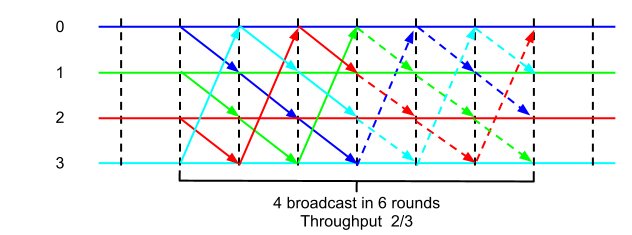
\includegraphics[width=280px]{Throughput2.png}
    \caption{Four nodes broadcasting on the pipeline. The dashed arrows are
    acknowledgements}
    \label{figure:throughput2}
\end{figure}

Finally, it take $2(N-1)$ rounds to broadcast $N$ messages, so we have a throughput
of $\frac{N}{2(N-1)}=\frac{1}{2-\frac{1}{N}}\longrightarrow_{N \rightarrow
\infty}\frac{1}{2}$. Two important point appears in that formula, the first is
that we have a lower bound for our throughput $\frac{1}{2}$. Secondly this limit 
is a constant so we can be sure that with a huge number of nodes our broadcast
will still be scalable.

\subsection{Empirical analysis}
\subsubsection{Latency}
As for the previous protocol, we recorded the latency $L$ for system with
different number of nodes. The results are shown in Table \ref{table:th}.

\begin{table}[H]
    \centering
    \begin{tabular}{|c|c|c|}
        \hline
        $N$   & L   & $2(N-1)$ \\
        \hline
        1     & 0   & 0    \\
        2     & 2   & 2   \\
        3     & 4   & 4   \\
        4     & 6   & 6   \\
        5     & 8   & 8   \\
        6     & 10  & 10  \\
        7     & 12  & 12  \\
        8     & 14  & 14  \\
        9     & 16  & 16  \\
        10    & 18  & 18  \\
        100   & 198 & 198  \\
        1000  & 1998   & 1998  \\
        %    10000 & 19998   & 19998  \\
        \hline
    \end{tabular}
    \caption{Protocol latency with different number of nodes.}
    \label{table:th}
\end{table}

We can see that the results correspond exactly to the theoretical analysis.

\subsubsection{Throughput}
To evaluate the throughput of the protocol, we ran an experiment with $N$
nodes, each node starting a broadcast at the first round. We recorded the
number of rounds needed for the $N$ broadcasts to finish, and used it to
compute the throughput $T$. The results are shown in Table \ref{table:thT}.

\begin{table}[H]
    \centering
    \begin{tabular}{|c|c|c|}
        \hline
        $N$   & T      & $2(N-1)$ \\
        \hline
        1     & +Inf   & +Inf   \\
        2     & 1      & 1      \\
        3     & 0.75   &  0.75  \\
        4     & 0.667  & 0.667  \\
        5     & 0.625  & 0.625  \\
        6     & 0.6    &   0.6  \\
        7     & 0.583  & 0.583  \\
        8     & 0.572  & 0.572  \\
        9     & 0.562  & 0.562  \\
        10    & 0.556  & 0.556  \\
        100   & 0.506  & 0.506  \\
        1000  & 0.500  & 0.500  \\
        %    10000 &   &   \\
        \hline
    \end{tabular}
    \caption{Protocol throughput with different number of nodes, all nodes broadcasting a message concurrently}
    \label{table:thT}
\end{table}

Once again, the results fit the theoretical model.

%%%%%%%%%%%%%%%%%%%%%%%%%%%%%%%%%%%%%%%%%%%%%%%%%%%%%%%%%%%%%%%%%%%%%%%%%%%%%%
\section*{Conclusion}
\addcontentsline{toc}{section}{Conclusion}
In this report we presented our implementation of a single-threaded,
round-based, network simulator. We later used it to implement and reason about
two total-order broadcast protocols that we designed.

One of them achieves a latency of $\lceil\log_2(N)\rceil + 1$ which is close
to the optimal latency that one can achieve with a broadcast protocol where no
total-order is required.

The second protocol achieves a throughput of $\frac{N}{2(N-1)}$ which has
$\frac{1}{2}$ as a lower bound. This result is quite far from the optimal
throughput for a broadcast protocol where no total order is required
($\frac{N+1}{N}$), but this is the price to pay to achieve a total ordering
of messages. However, since $\frac{1}{2}$ is a lower bound on the throughput
the performances of the protocol are scalable and become acceptable when
the number of nodes in the system is large.

An interesting future work would be to try to prove that there exists no
total-order broadcast protocol having latency lower than
$\lceil\log_2(N)\rceil + 1$. It would also be interesting to try to find
total-order protocols achieving a better throughput than the second protocol
presented in this report (if this is even possible).

\end{document}
